\setcounter{chapter}{3}
\renewcommand{\thechapter}{D}
\chapter{Diffusion}


\section{Introduction and Diffusion Equation}
We define \textbf{diffusion} as the transport of "stuff" (i.e. small particles, molecules dye, etc.) in a fluid without flow.

\paragraph{Remarks} Diffusion and convection transport often happen simultaneously. Chemical diffusion is a form of mass transport that is mathematically (but not physically) similar to heat conduction.

\subsection{A Microscopic Description of Diffusion}
Model: random walk on a 1D-lattice.
\begin{figure}[H]
	\centering
	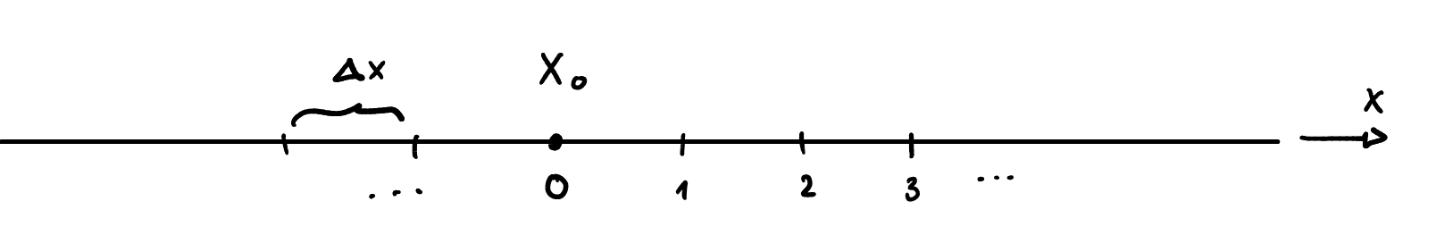
\includegraphics[width=0.7\linewidth]{Sketches/RandomWalk}
	%\caption{}
	\label{fig:randomwalk}
\end{figure}
we call $n(x,t)$ the number of particles at a position $x$ and time $t$ ("number density").

The change of $n$ in a time interval $\Delta t$ can be thought of as follows:

\begin{figure}[H]
	\centering
	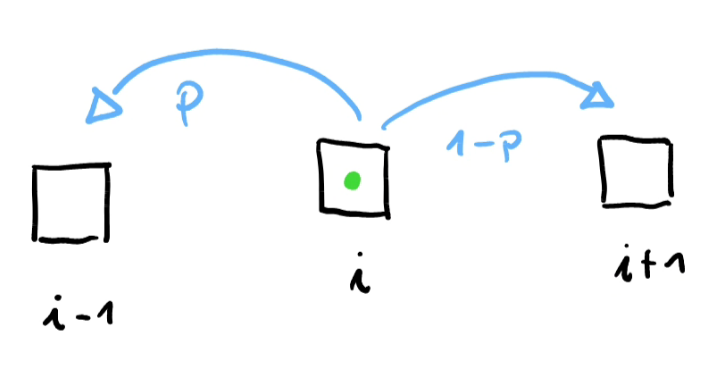
\includegraphics[width=0.3\linewidth]{Sketches/RandomWalkJumps}
	\caption{}
	\label{fig:randomwalkjumps}
\end{figure}

We assume that a particle jumps left with probability $p$ and towards the left with probability $1-p$. If $p=1/2$ we talk about an unbiased walk, when $p\ne 1/2$, it is a biased walk.

The change of particles in a time interval can be expressed as the outflow subtracted from the sum of influxes from the left and right:
\begin{equation}
	\Delta n \approx \frac{\partial n}{\partial t}\Delta t = n(x+\Delta x,t)p + n(x-\Delta x, t)(1-p)-n(x,t)
	\label{eq:diffusion_mass_conservation}
\end{equation}

This expression is just a discrete representation of mass conservation: No particle can get lost, they all have to go somewhere.

We treat $n(x,t)$ as continuous\footnote{Fishy, we know. This can also done by integrating formally to get a jump probability against time.} assuming that $\Delta x$s are really small and the amount of boxes is really large. We can therefore take a Taylor expansion:
\begin{equation*}
	\begin{split}
		n(x+\Delta x,t) = n(x)+\Delta x \frac{\partial n}{\partial x} + \frac{(\Delta x)^2}2 \frac{\partial ^2 n}{\partial x^2} + \dots \\
		n(x-\Delta x,t) = n(x)-\Delta x \frac{\partial n}{\partial x} + \frac{(\Delta x)^2}2 \frac{\partial ^2 n}{\partial x^2} + \dots \\
	\end{split}
\end{equation*}
which can be plugged into the equation \eqref{eq:diffusion_mass_conservation}:
\begin{equation*}
	\begin{split}
		\Delta n  &= \Delta x(p - (1-p))\frac{\partial n}{\partial x} + \frac{(\Delta x)^2}2\frac{\partial^2 n}{\partial x^2}+ \dots\\
		\frac{\partial n}{\partial t} &= -(1-2p)\frac{\Delta x}{\Delta t} \frac{\partial n}{\partial x} + \frac{(\Delta x)^2}{2\Delta t} \frac{\partial ^2 n}{\partial x^2}\qquad \left | \Delta x/ \Delta  t = v \right.\\
		\frac{\partial n}{\partial t} + v \frac{\partial n}{\partial x} &= D\frac{\partial ^2 n}{\partial x^2} \qquad \left | 
		\begin{cases}D = \frac{(\Delta x)^2}{2\Delta t} & \text{diffusion coefficient}\\ v=  (1-2p)\Delta x/\Delta t& \text{drift velocity}\end{cases}
		\right .
	\end{split}
\end{equation*}
For an unbiased random walk we pose $p=0.5$ which cancels the drift velocity. This makes the above turn into the well known \textbf{Diffusion Equation}:
\begin{equation}
	\boxed{\frac{\partial n}{\partial t} = D\frac{\partial ^2 n}{\partial x}}
	\label{eq:diffusion_1d}
\end{equation}
With the diffusion coefficient $D: [D]=m^2/s$

\paragraph{Remarks}
\begin{enumerate}
	\setlength{\itemsep}{-5pt}
	\item The net flux towards the left ($x+\Delta x \to x$) of an unbiased random walk is proportional to the gradient of the concentration $n$: $\frac 12 \Delta x \frac{\partial n}{\partial x} + \dots \propto \frac{\partial n}{\partial x}$.\\
	\item The same model applied for a 3D lattice yields a similar equation:$$\frac{\partial n}{\partial t}\ = D\nabla ^2n,\qquad D = \frac{\delta ^2}{6\Delta t}$$
	\item We can use this model to estimate diffusion coefficients: 
	\subitem Self diffusion: we know the velocity of a particle from statistical thermodynamics and can set $D \approx \frac \delta 6 \left(\frac{2k_b T}{m}\right)^{1/2}\approx 1.5\cdot 10^{-5} cm^2/s$ which is very exact.
	\subitem Suspended particles: A sphere of radius $a$ in a liquid with viscosity $\mu$ has a coefficient $D=\frac{k_BT}{6\pi \mu a}$, which is the Stokes-Einstein relation.
\end{enumerate}



\subsection{A Continuum Description of Diffusion}

We consider a concentration field $c(\vec x,t)$ of units $m^{-3}$. We start with the observation that molecules diffuse from higher to lower concentrations, which is expressed in \textbf{Fick's Law}:
\begin{equation}
	\boxed{\vec j = -D\nabla c}
	\label{eq:ficks_law}
\end{equation}

where $\vec j$ is the number flux: $\frac{1}{\mathrm{time}\cdot \mathrm{area}}$

\begin{figure}[H]
	\centering
	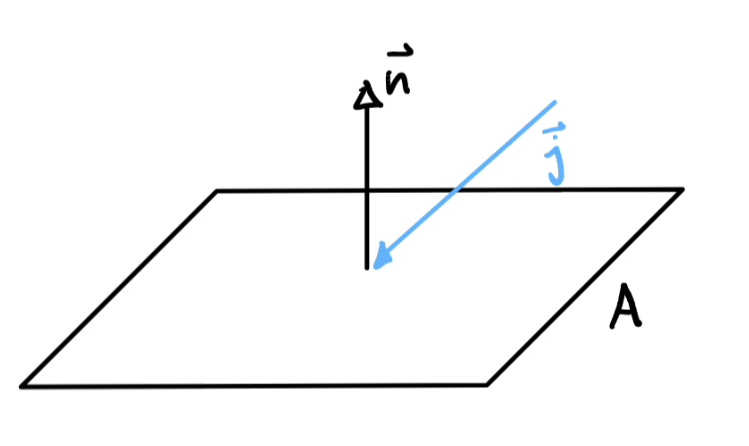
\includegraphics[width=0.3\linewidth]{Sketches/FicksLaw}
	%\caption{}
	\label{fig:fickslaw}
\end{figure}

The number of molecules transported trough area $A$ per time is
\begin{equation*}
	\int_A \vec j \cdot \hat n \, dA
\end{equation*}


Mass conservation in a control volume states, that the rate of change of "stuff" inside is the rate that goes out subtracted from the rate that goes in:
\begin{equation*}
	\begin{split}
	\frac \partial {\partial t}\left[\int_V c\,dV\right] &= -\oint_S \vec j \cdot \,d\vec S\\
	&\stackrel{(*)}{=} \int_V \nabla \cdot \vec j \,dV\\
	\int_V\frac{\partial c}{\partial t}\,dV &= -\int_V \nabla \cdot \vec j \,dV\\
	\int_V\frac{\partial c}{\partial t}- \nabla \cdot \vec j \,dV &= 0\\
	\end{split}
\end{equation*}
where at $(*)$ we used Gauss's law. The volume $V$ is arbitrary, so the above statement is true for all volumes $V$. This is only true, if the integrand is also zero. This leads to a representation of mass conservation in the general form of a differential conservation law:
\begin{equation*}
	\frac{\partial}{\partial t} c + \nabla \cdot \vec j = 0
\end{equation*}

Plugging in Fick's law ($\vec j = -D\nabla c$), we get
\begin{equation*}
	\frac{\partial}{\partial t}c = \nabla (D\nabla c)
\end{equation*}

For $D=const$ we get the \textbf{diffusion equation} from before:
\begin{equation}
	\boxed{\frac{\partial c}{\partial t} = D \nabla^2 c}
\end{equation}

\paragraph{Remarks}

\begin{enumerate}
	\setlength{\itemsep}{-5pt}
	\item The equation results in \eqref{eq:diffusion_1d} in one dimension.
	\item Heat conduction is derived by combining conservation of energy and Fourrier's-Law for chemical energy flux, yielding $\frac{\partial T}{\partial t} = \kappa \nabla ^2 T$ where $\kappa= k/\rho c_p$ is the thermal diffusivity.
	\item The diffusion equation is a partial differential equation (PDE) which needs to be solved with the initial condition (initial concentration) and boundary conditions such as
	\subitem the concentration
	\subitem the flux  $\hat n \cdot \vec j = -D\hat n  \cdot \nabla c$
	\subitem a mix: linked flux with surface concentration (e.g. $\gamma = h(c-c_\infty)$)
\end{enumerate}
 

\section{Solving the Diffusion Equation at Steady State}
\subsection{One Dimensional Linear Problem}
We consider the following system: Two tanks with respective constant concentration $\alpha$ and $\beta$ are connected through a thin pipe of length $l$.
\begin{figure}[H]
	\centering
	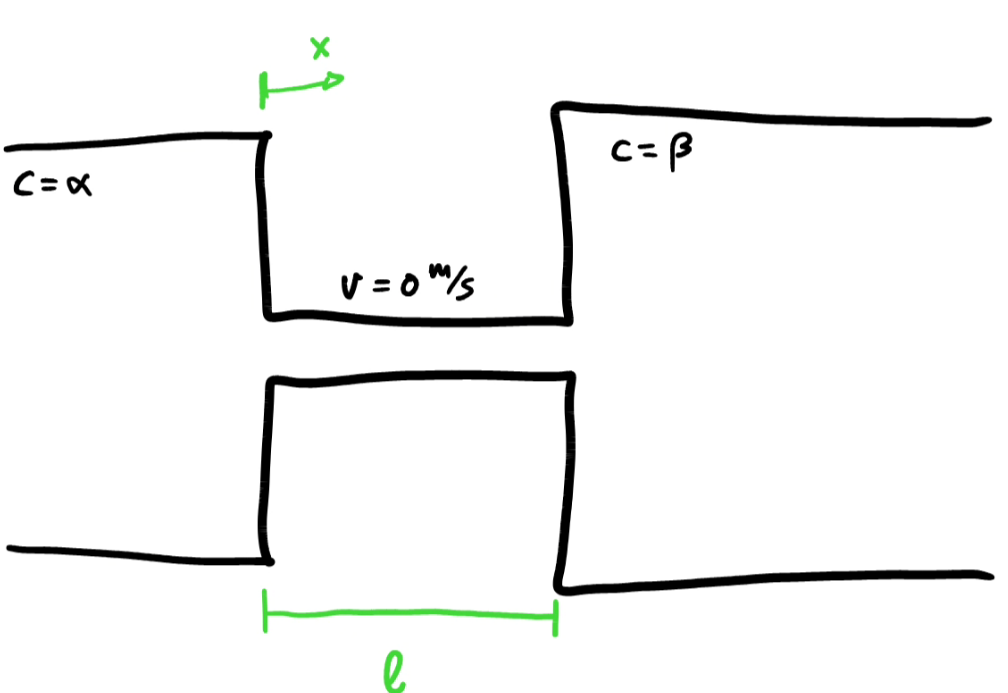
\includegraphics[width=0.5\linewidth]{Sketches/TanksDiffusion}
	%\caption{}
	\label{fig:tanksdiffusion}
\end{figure}

We approximate the pipe as a 1D system, with this we can express the concentration as follows:
\begin{equation*}
	\frac{\partial c}{\partial t} = D\frac{\partial ^2 c}{\partial x^2},\qquad c(x,t),\qquad 0\le 0 \le L
\end{equation*}
We state the boundary conditions:
\begin{equation*}
	\left.\begin{split}
		c(x=0,t)= \alpha\\
		c(x=L,t)= \beta
	\end{split}\right\} \text{Dirichlet Type}
\end{equation*}
At steady state, we know that $\frac{\partial c}{\partial t} = 0$. With these values, there is no initial condition required:
\begin{equation*}
	\begin{split}
		D\frac{\partial ^2 c}{\partial x^2} &= 0\qquad \text{ODE}\\
		c(x) &= A_1x+A_2\\
		\implies &\begin{cases}
			A_1\cdot 0 + A_2 = \alpha\\
			A_1\cdot L + A_2 = \beta
		\end{cases}\\
		c(x) &= \frac{\beta- \alpha}{L}x + \alpha
	\end{split}
\end{equation*}


\paragraph{Notes} The result is unique. It is independent of $D$ because we are assuming steady state, there are no rates.

\subsection{Spherical Problem}

We have two spheres of chemicals and want to find the concentration distribution at steady state.
\begin{figure}[H]
	\centering
	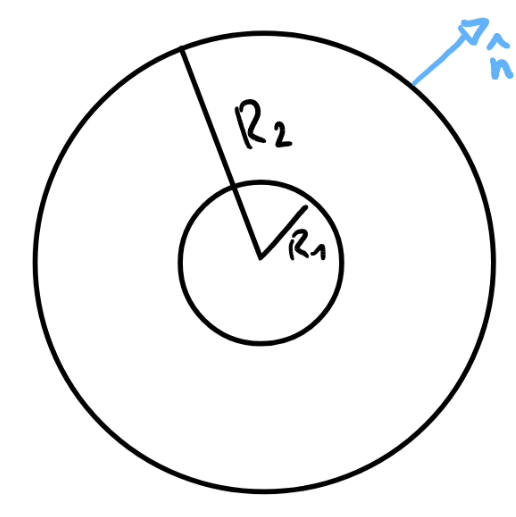
\includegraphics[width=0.4\linewidth]{Sketches/SpheresDiffusion}
	%\caption{}
	\label{fig:spheresdiffusion}
\end{figure}

\begin{equation*}
	\cancel{\frac{\partial c}{\partial t}}^0 = D\nabla ^2 c
\end{equation*}
with the boundary condition of the flux $\vec j \cdot \hat n = -\alpha @ R_2$ and the concentration at $R_1$ is $0$.

If we were to apply the laplacien in cartesian coordinates, we would have difficulties expressing everything, as our system has spherical symmetries, we are better off using the spherical laplacien:
\begin{equation*}
	\nabla^2c = \frac 1{r^2}\frac\partial {\partial r}\left(r^2\frac{\partial c}{\partial r}\right) + \frac 1{r^2\sin\theta}\frac{\partial}{\partial \theta}\left(\sin\theta \frac{\partial c}{\partial \theta}\right) + \frac 1{r^2\sin\theta}\frac{\partial ^2c}{\partial \varphi^2}
\end{equation*}
Through symmetry we know that $c$ is a function of $r$, therefore $\frac{\partial c}{\partial \theta}=\frac{\partial c}{\partial \varphi}=0$. This makes a lot of the terms from the laplacien disappear. What is left is:
\begin{equation*}
	\nabla^2c = \frac 1{r^2}\frac\partial {\partial r}\left(r^2\frac{\partial c}{\partial r}\right)
\end{equation*}
From here we combine the diffusion equation with the laplacien:
\begin{equation*}
	\begin{split}
		0 &= \frac{1}{r^2}\frac{\partial}{\partial r} \left(r^2 \frac{\partial}{\partial r}c\right)\\
		0&=\frac{1}{r^2}\frac{d}{dr}\left(r^2\frac{d}{dr}c\right)\\
		r^2\frac d{dr} c &= A_1\\
		c &= -\frac{A_1}r + A_2\quad
		\begin{cases}
			c(R_1)=0\\
			D\frac{\partial c}{\partial r}\Big|_{R_2} = \alpha\\
			\vec{j} = -D\nabla c
		\end{cases}\\
		\implies & \begin{cases}
		c(r=R_1) = -\frac{A_1}{R_1} + A_2 = 0\\
		D\frac{\partial c}{\partial r}\Big|_{R_2}= D\frac{A_1}{R_2^2}  =\alpha
		\end{cases}\implies \begin{cases}
		A_1=\frac {\alpha R_2^2}{D}\\
		A_2= \frac{\alpha R_2^2}{DR_1}
		\end{cases}\\
		c(r)&=-\frac{\frac {\alpha R_2^2}{D}}{r} + \frac{\alpha R_2^2}{DR_1}\\
		&= \frac{\alpha R_2^2}{D}\left(\frac 1{R_1}-\frac 1{r}\right)
	\end{split}
\end{equation*}

Which looks something like the following plot, plotting for $x\in[R_1,R_2]$:
\begin{figure}[H]
	\centering
	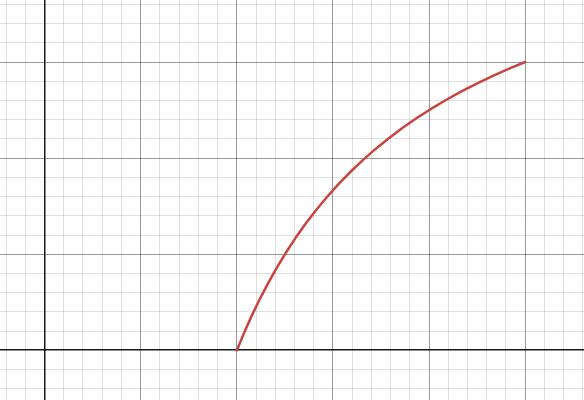
\includegraphics[width=0.4\linewidth]{Sketches/SpheresDiffusionPlot}
	
	\label{fig:spheresdiffusionplot}
\end{figure}

\paragraph{Notes}
This equation is also valid for steady-state with sources and sinks:
\begin{equation*}
	\frac{\partial c}{\partial t} = D \nabla^2c+f
\end{equation*}
where $f$ is for example some chemical reaction ($f=-\alpha$, or $f=-kc$)


\section{Solving the Diffusion Equation with Time Dependency}

\subsection{Finite one Dimensional Domain (Series Expansions)}
\subsubsection{Fixed Concentration}

We pose a partial differential equations the following with boundary conditions and initial conditions:
\begin{equation*}
	\frac{\partial c}{\partial t} = D\frac{\partial^2 c}{\partial x^2}
	\qquad c(x=0,t)=c(x=L,t)=0\qquad c(x,t=0)=c_0(x)
\end{equation*}
Which is a linear and homogenous PDE  with homogeneous boundary conditions.
Therefore if $c_1(x,t)$ and $c_2(x,t)$ are two solutions then $(c_1+c_2)(x,t)$ and $(\beta c_1)(x,t), \beta \in \mathbb R$ are also solutions\footnote{This allows us to look for simple solutions and then construct a sum of the simpler solutions that satisfies the initial conditions.}. Note that this only works for homogeneous boundary conditions. 
The approach is based on linearity: 

\paragraph{Step 1: Write a General Solution} At first, we write a general solution of the PDE with boundary conditions as a linear combination of so-called \textit{base solutions}:
\begin{equation*}
	c(x,t)  = \sum_{n=1}^\infty A_n\varphi_n(x,t)
\end{equation*}
where $\varphi_n$ are simple \textit{base solutions} and $A_n$ are \textit{expansion coefficients}.

\paragraph{Step 2: Determine the Expansion Coefficients} As a second step, we want to determine $\{A_n\}$ such that $c(x,t)$ satisfies the initial condition:
\begin{equation*}
	c(x,t=0)=c_0(x)
\end{equation*}

We start by trying to find any solution, we call \textit{base solution} $\varphi$. We try this by applying separation of variables, assuming $\varphi(x,t)=X(x)T(t)$\footnote{There is no guarantee that we can find a solution of this type. It is an attempt: If I try this, will i find a solution?}. We insert this function into our PDE:
\begin{equation*}
	\begin{split}
		\frac{\partial \varphi}{\partial t} &= D \frac{\partial^2 \varphi}{\partial x^2}\\
		X(x)\frac{dT(t)}{dt}&=DT(t)\frac{d^2 X(x)}{dx^2}\\
		X(x)T'(t)&=DT(t)X''(x)\\
		\frac 1D \frac{T'(t)}{T(t)} &= \frac{X''(x)}{X(x)} \stackrel{(*)}{=}-\lambda\\
	\end{split}
\end{equation*}
Since both sides are independent of each other (left hand side is a function of time, the right hand side is a function of position), it must be equal to a constant $-\lambda$ at $(*)$
The above yields two ordinary differential equations, coupled by an unknown $\lambda$:
\begin{equation*}
		T'(t)+ D\lambda T(t) = 0
		\qquad
		X''(t) + \lambda X(t) = 0
\end{equation*}
The boundary conditions of before still apply:
\begin{equation*}
	\begin{cases}
		\varphi(x=0, t) = 0\\
		\varphi(x=L, t) = 0\\
	\end{cases}\implies
	\begin{cases}
		X(0)=X(L) = 0
	\end{cases}
\end{equation*}
Since the conditions only apply to the spatial equation, we start by solving for $X(t)$, then try to apply our findings to the temporal problem.

We solve $X''(t)+\lambda X(t) = 0$, depending on the sign of $\lambda$ as follows:
\begin{equation*}
	\begin{split}
		\text{Case 1: $\lambda < 0$}: \qquad 
		X(x) & = \alpha_1 e^{{\sqrt-\lambda}x}+ \alpha_2 e^{-\sqrt{-\lambda}x}\\
		 	 & \stackrel{(*)}{=} 0\\
		\text{Case 2: $\lambda = 0$}: \qquad X(x) &= \alpha_1 x + \alpha_2\\
		 	 & \stackrel{(**)}{=} 0\\
		\text{Case 3: $\lambda > 0$}: \qquad X(x) &= \alpha_1 \cos(\sqrt \lambda x) + \alpha_2 \sin(\sqrt \lambda x) \qquad \left | X(0) = 0 \implies \alpha_1 = 0\right .\\
		X(L)&= \alpha_2 \sin(\sqrt \lambda L) = 0\text{ and }\alpha_2 \ne 0\Leftrightarrow \lambda = \left(\frac{\pi n}{L}\right)^2\\
		X(x) &= \alpha_2 \sin\left(\frac{n\pi x}{L}\right)\qquad n \in \mathbb N
	\end{split}
\end{equation*}
At $(*)$ we have reduced the two linearly non-independent solutions and know that $\alpha_1=\alpha_2= 0$, only the trivial solution $X(x)=0$ is found. At $(**)$ we applied the boundary conditions and found the same trivial solution.
An infinite amount of solutions are found for the case where $\lambda > 0$.

Spatial base solutions are those sine/cosine terms which are compatible with the boundary conditions. The boundary conditions determine the coupling constants $\lambda_n$, which we call the eigenvalues of our problem. We now apply this to the temporal problem for a $\lambda_n = \left(\frac{\pi n}{L}\right)^2$:
\begin{equation*}
	\begin{split}
		T_n' &= -D\lambda_n T_n\\
		T_n(T)&=\beta_n e^{-D\lambda_m t} = \beta_n e^{-D\left(\frac{\pi n}{L}\right) ^2 t}
	\end{split}
\end{equation*}
We recognize the solution $T_n$ as a decaying exponential. The combined solution $\varphi$ can be expressed as:
\begin{equation*}
	\varphi_n(x,t) = e^{-D\left(\frac{\pi n}{L}\right) ^2 t} \sin\left(\frac{n\pi x}{L}\right)\qquad n \in \mathbb N\\
\end{equation*}
Through linearity, we were allowed to normalize the solutions and set $\alpha_n \cdot \beta_n = 1$.
The general solution of the PDE that satisfy the boundary conditions can be expressed as:
\begin{equation*}
	c(x,t)= \sum_{n=1}^\infty A_n e^{-D\left(\frac{\pi n}{L}\right) ^2 t} \sin\left(\frac{n\pi x}{L}\right)
\end{equation*}
We now want to determine $\{A_n\}$ from the initial conditions. We need to satisfy:
\begin{equation*}
	c_0(x) = c(x,t=0) = \sum_{n=1}^\infty A_n \sin\left(\frac{n\pi x}{L}\right)
\end{equation*}
Multiplying with one base solution (e.g. $\sin\frac{\pi mx}{L}$ with some integer $m$) and then integrate in $x$:
\begin{equation*}
	\begin{split}
		\int_0^L c_0(x)\sin\left(\frac{\pi m}{L}x \right) \,dx &= \sum_{n=1}^\infty A_n\int_0^L\sin\left(\frac{\pi n}{L} x \right)\sin\left(\frac{\pi m}{L} x \right)\,dx\\
		&\stackrel{(*)}{=}  \sum_{n=1}^\infty A_n\begin{cases}
			0 & n\ne m\\
			L/2 & n=m
		\end{cases}\\
		& = A_n \frac L2\\
		A_n & =\frac 2L \int_0^L c_0(x)\sin\left(\frac{\pi_n}Lx\right)\,dx
	\end{split}
\end{equation*}
At $(*)$ we use the fact that the integral over a common multiple of a period of two sines or cosines with different frequencies yields 0. \footnote{This can be shown using the identity $\sin a \sin b = \frac 12(\cos(a-b)-\cos(a+b))$ over a full period.}

Through Fourier's theorems, we know that any smooth initial condition satisfying my boundary conditions can be expressed as a sine, cosine or Fourier series, meaning we have the complete solution. For any $c_0(x)$, the complete solution is:
\begin{equation}
	\boxed{c(x,t) = \sum_{n=1}^\infty \underbrace{\left[ \frac 2L \int_0^L c_0(\tilde  x)\sin\left(\frac{\pi n}L\tilde x\right)\,d\tilde x\right]}_{\text{expansion coefficient of mode}} \underbrace{e^{-D\left(\frac{\pi n}{L}\right)^2x}}_{\text{time evolution}}\underbrace{\sin\left(\frac{\pi n}{L} x\right)}_{\text{spatial mode}}}
\end{equation}
\setcounter{chapter}{4}
\renewcommand{\thechapter}{\arabic{chapter}}


